\documentclass[11pt, a4paper]{article}
\usepackage[utf8]{inputenc}
\usepackage[margin=1in]{geometry} %Sets proper 1-inch margins. 
\usepackage{amsmath} %Only load this if you are using math/equations.
\usepackage{graphicx} %Only need to call this if inserting images.
\usepackage{caption} %Only need to call this if inserting captions.
\usepackage{float} %Allows the use of the [H] specifier. 
\graphicspath{{C:/Users/jonah/Pictures/meme/}} %Sets the working directory for images.
\usepackage[colorlinks,citecolor=blue,linkcolor=blue,urlcolor=blue]{hyperref} %Allows for the embedding of urls. 
\usepackage{setspace}
\usepackage{blindtext}

\pagenumbering{arabic}

\usepackage{fancyhdr}

\pagestyle{fancy}
\fancyhf{}
\rhead{Jonah Edmundson \\ 2023}
\lhead{\thepage}

\newcommand{\comment}[1]{}

\usepackage{Sweave}
\begin{document}
\Sconcordance{concordance:variableinvestigation.tex:variableinvestigation.Rnw:%
1 23 1 1 0 19 1 1 2 1 0 3 1 1 6 5 0 1 3 1 0 1 3 1 0 1 12 14 0 1 2 8 1 1 %
3 2 0 1 2 1 0 1 2 1 0 1 2 6 0 1 6 9 0 1 2 3 1 1 4 3 0 1 2 8 0 1 7 9 0 1 %
2 6 1 1 2 1 0 1 7 9 0 1 2 1 5 10 0 1 8 11 0 1 2 2 1 1 14 17 0 1 2 30 1}


\begin{center}
\Large{\textsc{Variable Investigation}}
\par
\normalsize{\textsc{for}}
\par
\large{\textsc{Kelowna Weather-Crash Project}}
\end{center}


\vspace{0.917 pc} %Creates a paragraph line break. 

\tableofcontents


\pagebreak
%\section{Loading data}



\section{Summary Statistics}

\begin{Schunk}
\begin{Soutput}
Need to remove dew point temp and wind chill, 
since they are so correlated with temperature.
\end{Soutput}
\begin{Soutput}
                    Temp...C. Dew.Point.Temp...C. Wind.Chill
Temp...C.           1.0000000           0.9209662  0.9517406
Dew.Point.Temp...C. 0.9209662           1.0000000  0.9312014
Wind.Chill          0.9517406           0.9312014  1.0000000
\end{Soutput}
\begin{Soutput}
Summary of all variables:
\end{Soutput}
\begin{Soutput}
    linker          Date.Of.Loss.Year Animal.Flag              Crash.Severity 
 Length:56136       Min.   :2017      No :54118   CASUALTY CRASH      :11473  
 Class :character   1st Qu.:2018      Yes: 2018   PROPERTY DAMAGE ONLY:44663  
 Mode  :character   Median :2019                                              
                    Mean   :2019                                              
                    3rd Qu.:2020                                              
                    Max.   :2021                                              
                                                                              
 Cyclist.Flag    Day.Of.Week                Derived.Crash.Configuration
 No :55725    FRIDAY   :9316   REAR END                   :13024       
 Yes:  411    MONDAY   :8024   SINGLE VEHICLE             :12495       
              SATURDAY :6753   UNDETERMINED               :11453       
              SUNDAY   :5464   SIDE IMPACT                :11369       
              THURSDAY :9061   CONFLICTED                 : 3068       
              TUESDAY  :8728   SIDE SWIPE - SAME DIRECTION: 1833       
              WEDNESDAY:8790   (Other)                    : 2894       
 Heavy.Veh.Flag Intersection.Crash  Month.Of.Year   Motorcycle.Flag
 No :54085      No :31677          JULY    : 5152   No :55673      
 Yes: 2051      Yes:24459          DECEMBER: 5095   Yes:  463      
                                   JANUARY : 5063                  
                                   AUGUST  : 4907                  
                                   OCTOBER : 4836                  
                                   JUNE    : 4735                  
                                   (Other) :26348                  
 Parked.Vehicle.Flag Parking.Lot.Flag Pedestrian.Flag     Time.Category  
 No :38567           No :37189        No :55790       12:00-14:59:14870  
 Yes:17569           Yes:18947        Yes:  346       15:00-17:59:14473  
                                                      09:00-11:59:11021  
                                                      18:00-20:59: 5805  
                                                      06:00-08:59: 5489  
                                                      21:00-23:59: 2684  
                                                      (Other)    : 1794  
    Municipality.Name Road.Location.Description       Street.Full.Name
 KELOWNA     :45943   UNKNOWN     : 2211        HWY 97        : 6019  
 WEST KELOWNA:10193   HWY 97      : 1961        HARVEY AVE    : 3168  
                      HARVEY AVE  : 1670        HWY 33        : 2064  
                      LAKESHORE RD:  932        GORDON DR     : 1921  
                      LOUIE DR    :  751        LAKESHORE RD  : 1372  
                      HWY 33      :  715        SPRINGFIELD RD: 1326  
                      (Other)     :47896        (Other)       :40266  
 Total.Crashes   Total.Victims      Temp...C.       Rel.Hum....    
 Min.   :1.000   Min.   :0.0000   Min.   :-22.43   Min.   : 12.67  
 1st Qu.:1.000   1st Qu.:0.0000   1st Qu.:  1.60   1st Qu.: 38.00  
 Median :1.000   Median :0.0000   Median : 10.37   Median : 62.00  
 Mean   :1.006   Mean   :0.2917   Mean   : 10.92   Mean   : 60.51  
 3rd Qu.:1.000   3rd Qu.:0.0000   3rd Qu.: 20.00   3rd Qu.: 82.33  
 Max.   :3.000   Max.   :9.0000   Max.   : 37.73   Max.   :100.00  
                                  NA's   :35       NA's   :35      
 Precip..Amount..mm. Wind.Dir..10s.deg. Wind.Spd..km.h.  Visibility..km.
 Min.   :0.00000     Min.   : 1.00      Min.   : 0.000   Min.   : 0.20  
 1st Qu.:0.00000     1st Qu.:15.67      1st Qu.: 4.667   1st Qu.:16.10  
 Median :0.00000     Median :19.50      Median : 8.000   Median :16.10  
 Mean   :0.03111     Mean   :21.16      Mean   :10.277   Mean   :15.15  
 3rd Qu.:0.00000     3rd Qu.:31.00      3rd Qu.:13.667   3rd Qu.:16.10  
 Max.   :4.00000     Max.   :36.00      Max.   :51.333   Max.   :16.10  
 NA's   :35          NA's   :4020       NA's   :35       NA's   :36     
 Stn.Press..kPa. Fog       Freezing.Rain Snow      Rain      Thunderstorms
 Min.   :94.08   0:52106   0:56134       0:52325   0:50075   0:56002      
 1st Qu.:96.10   1: 4030   1:    2       1: 3811   1: 6061   1:  134      
 Median :96.51                                                            
 Mean   :96.56                                                            
 3rd Qu.:96.90                                                            
 Max.   :99.33                                                            
 NA's   :35                                                               
\end{Soutput}
\end{Schunk}
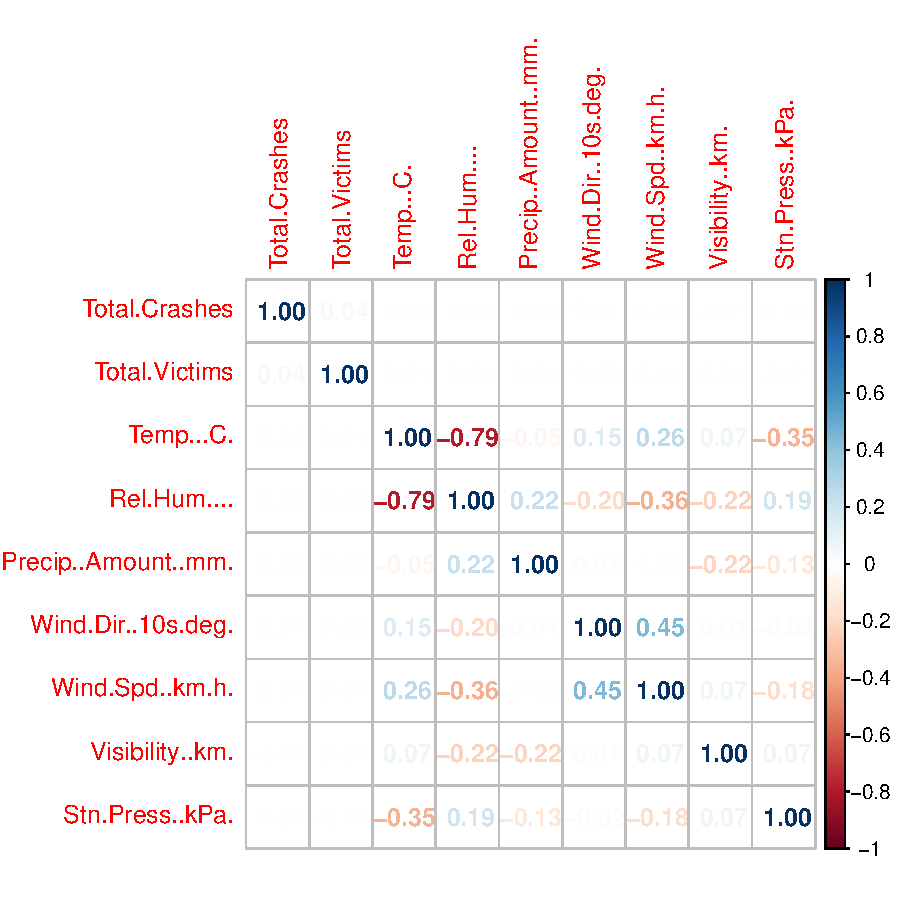
\includegraphics{variableinvestigation-ss}




\pagebreak
\section{Accidents over Time}

\subsection{Throughout the Day}

\begin{Schunk}
\begin{Soutput}
00:00-02:59 03:00-05:59 06:00-08:59 09:00-11:59 12:00-14:59 15:00-17:59 
        977         817        5489       11021       14870       14473 
18:00-20:59 21:00-23:59 
       5805        2684 
\end{Soutput}
\end{Schunk}
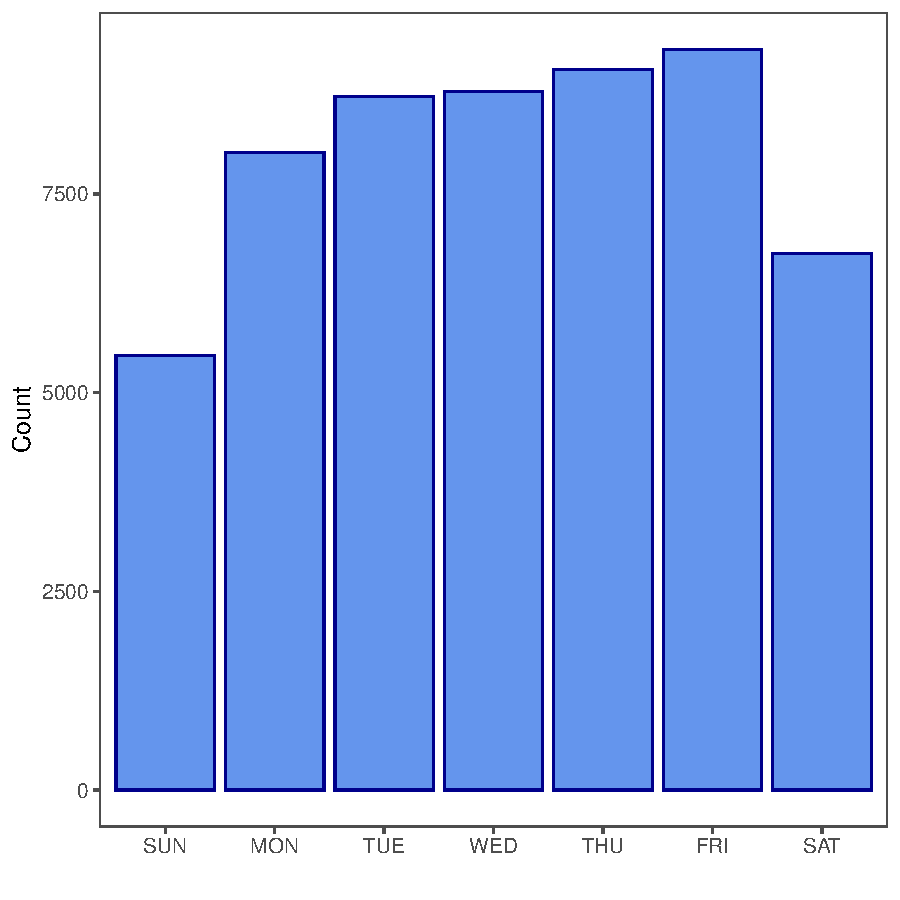
\includegraphics{variableinvestigation-003}


\pagebreak
\subsection{Day of the Week} 

Distribution of accidents throughout the week:

\begin{Schunk}
\begin{Soutput}
   SUNDAY    MONDAY   TUESDAY WEDNESDAY  THURSDAY    FRIDAY  SATURDAY 
     5464      8024      8728      8790      9061      9316      6753 
\end{Soutput}
\end{Schunk}
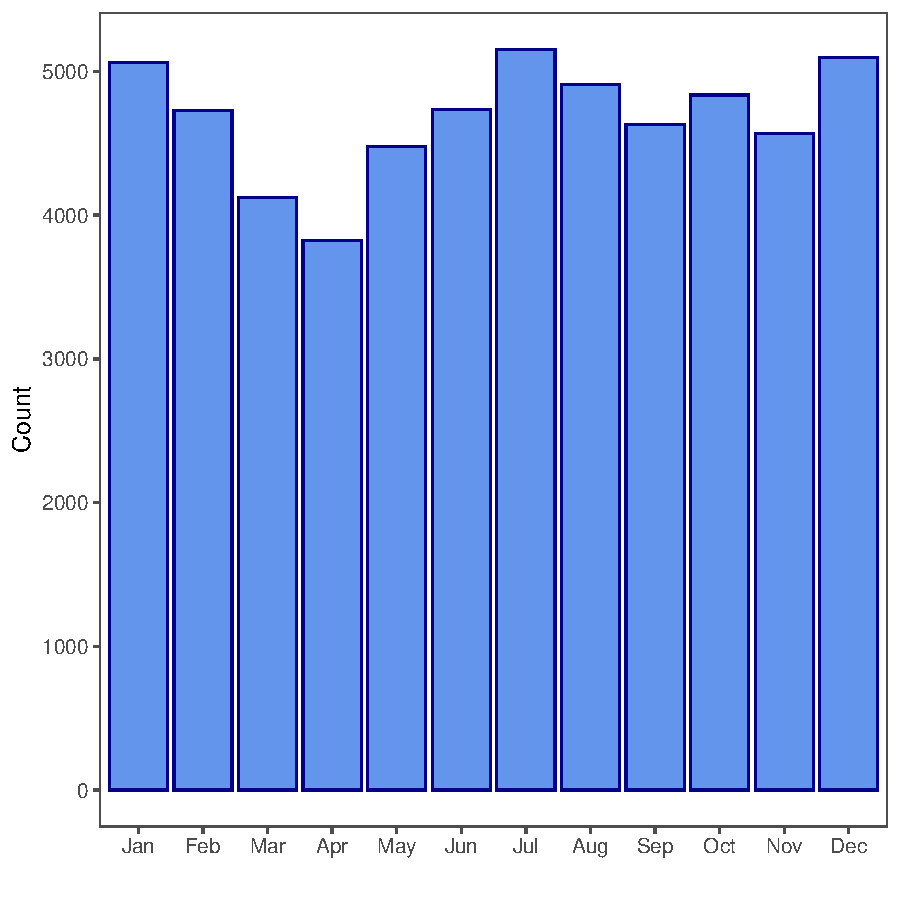
\includegraphics{variableinvestigation-004}


\pagebreak
\subsection{Month of the Year}

\begin{Schunk}
\begin{Soutput}
  JANUARY  FEBRUARY     MARCH     APRIL       MAY      JUNE      JULY    AUGUST 
     5063      4728      4120      3825      4475      4735      5152      4907 
SEPTEMBER   OCTOBER  NOVEMBER  DECEMBER 
     4632      4836      4568      5095 
\end{Soutput}
\end{Schunk}
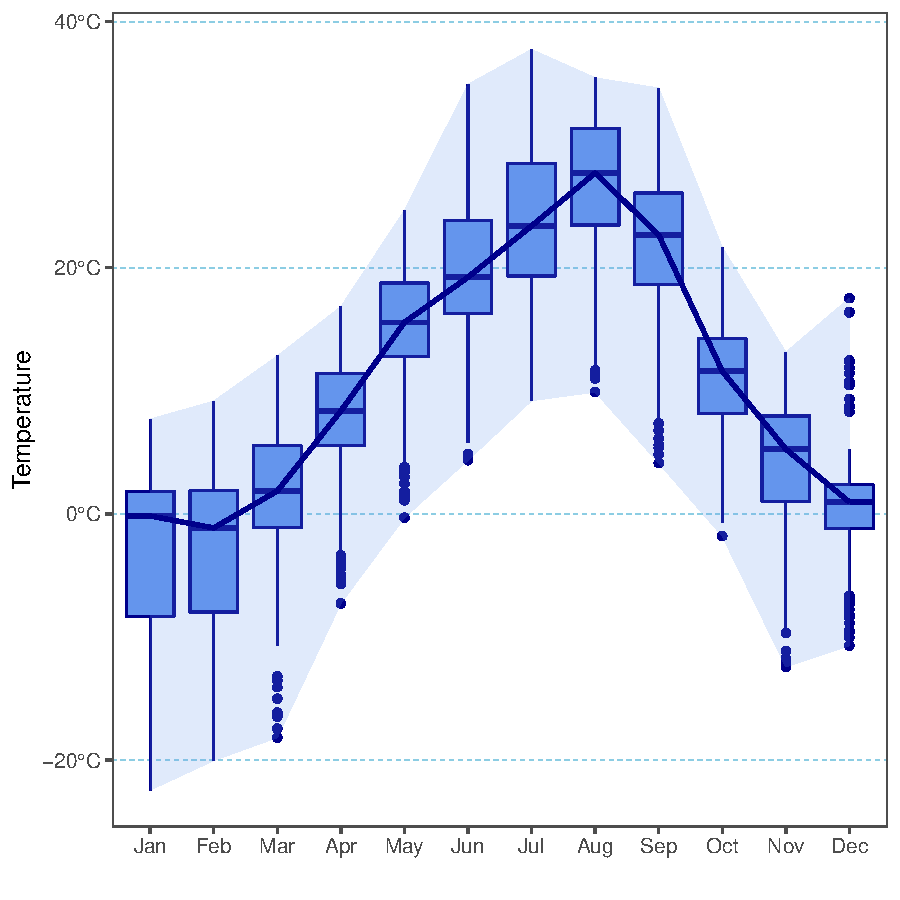
\includegraphics{variableinvestigation-005}


\pagebreak
\subsection{Over the Years}

\begin{Schunk}
\begin{Soutput}
 2017  2018  2019  2020  2021 
12734 12324 11148  9275 10655 
\end{Soutput}
\end{Schunk}
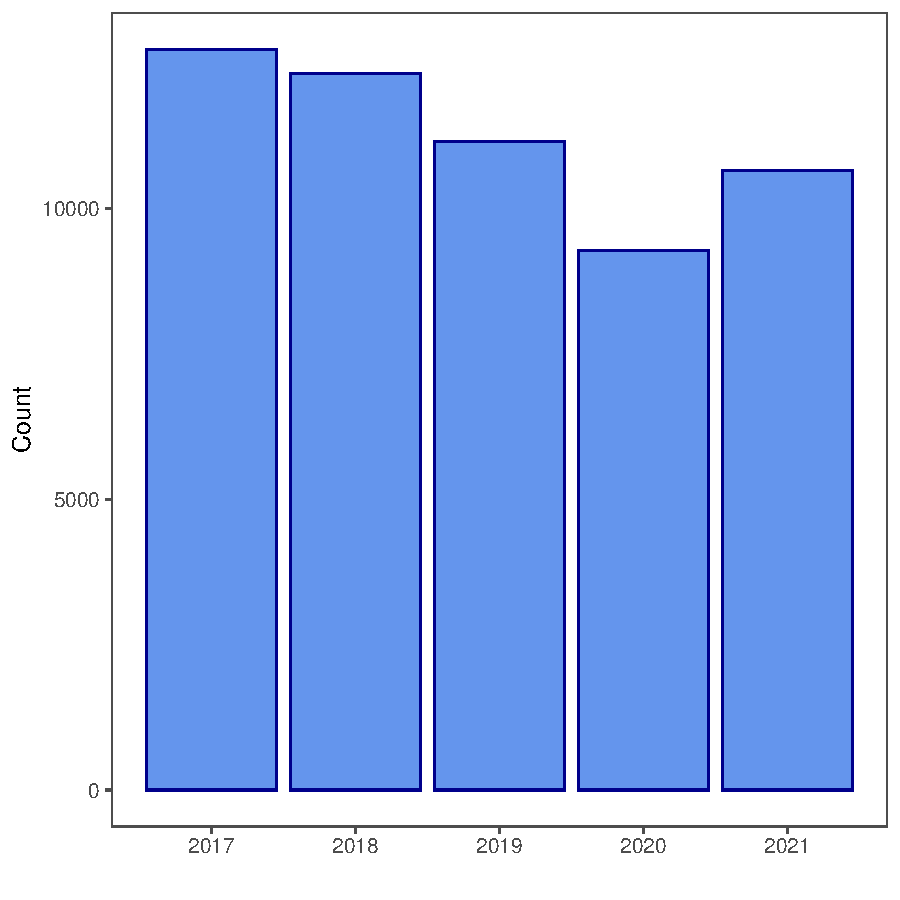
\includegraphics{variableinvestigation-006}





\pagebreak
\section{Distributions of Weather Variables}

\subsection{Temperature}


\begin{Schunk}
\begin{Soutput}
  Avg.temp. Avg.crash.temp.
1  8.511442        10.91872
\end{Soutput}
\end{Schunk}
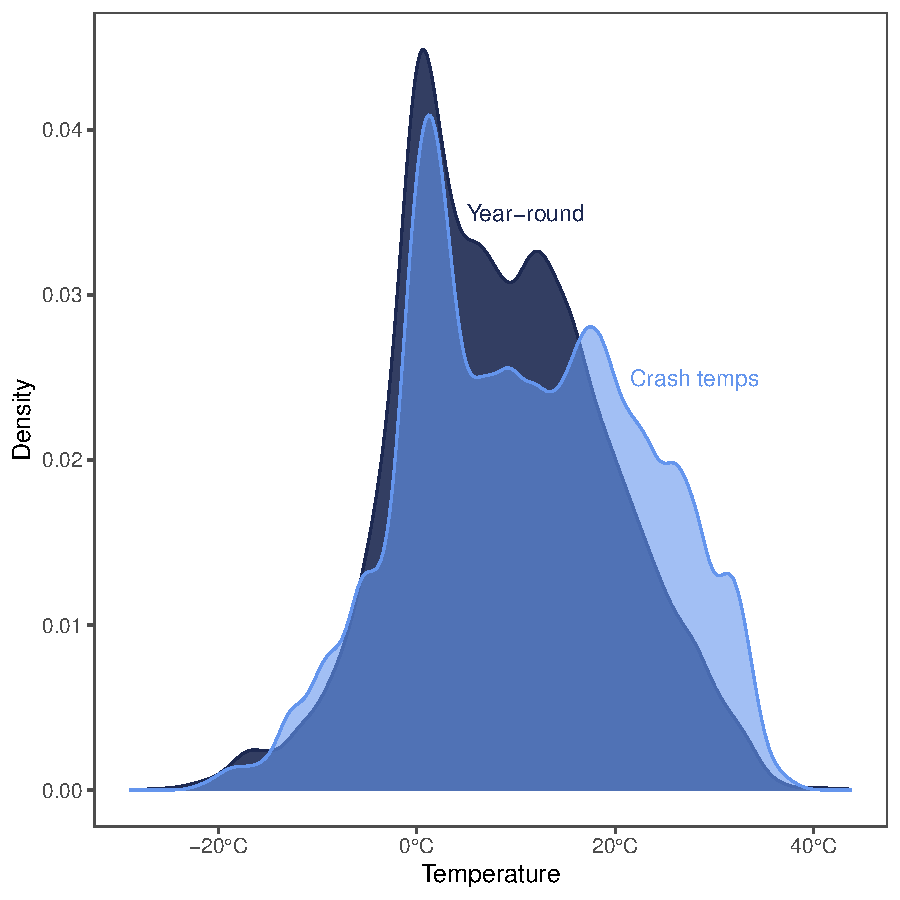
\includegraphics{variableinvestigation-008}



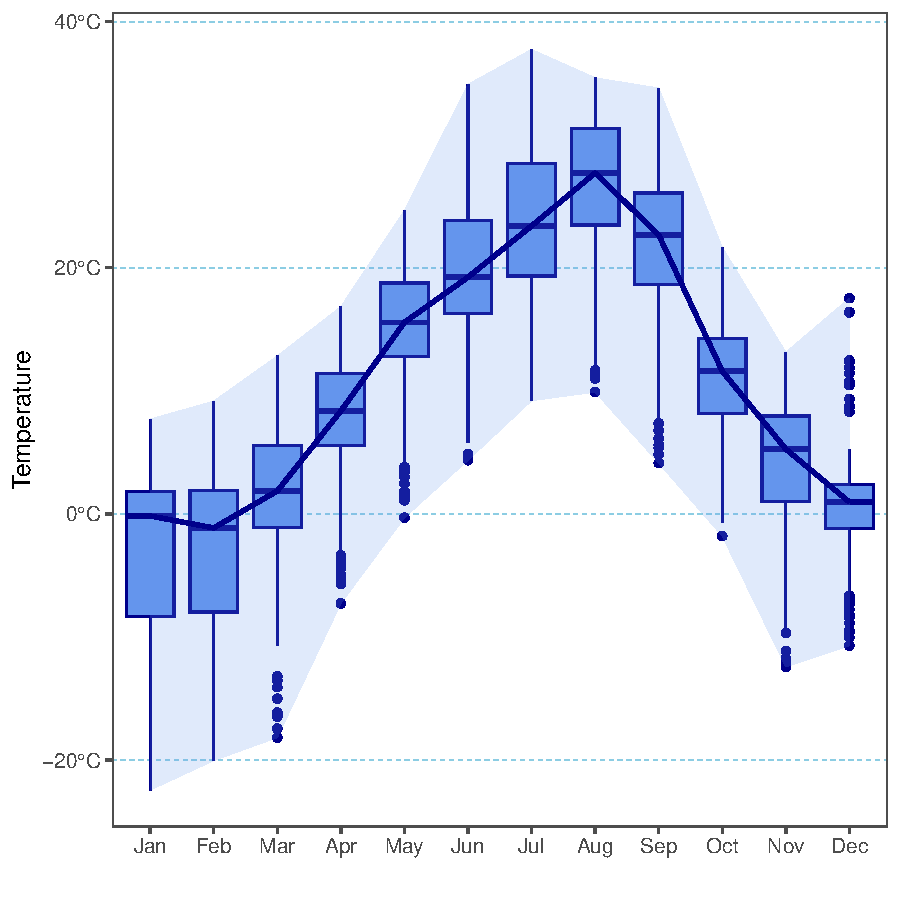
\includegraphics{variableinvestigation-009}



\pagebreak
\subsection{Relative Humidity}

\begin{Schunk}
\begin{Soutput}
  Avg.humidity Avg.crash.humidity
1     69.32555           60.50743
\end{Soutput}
\end{Schunk}
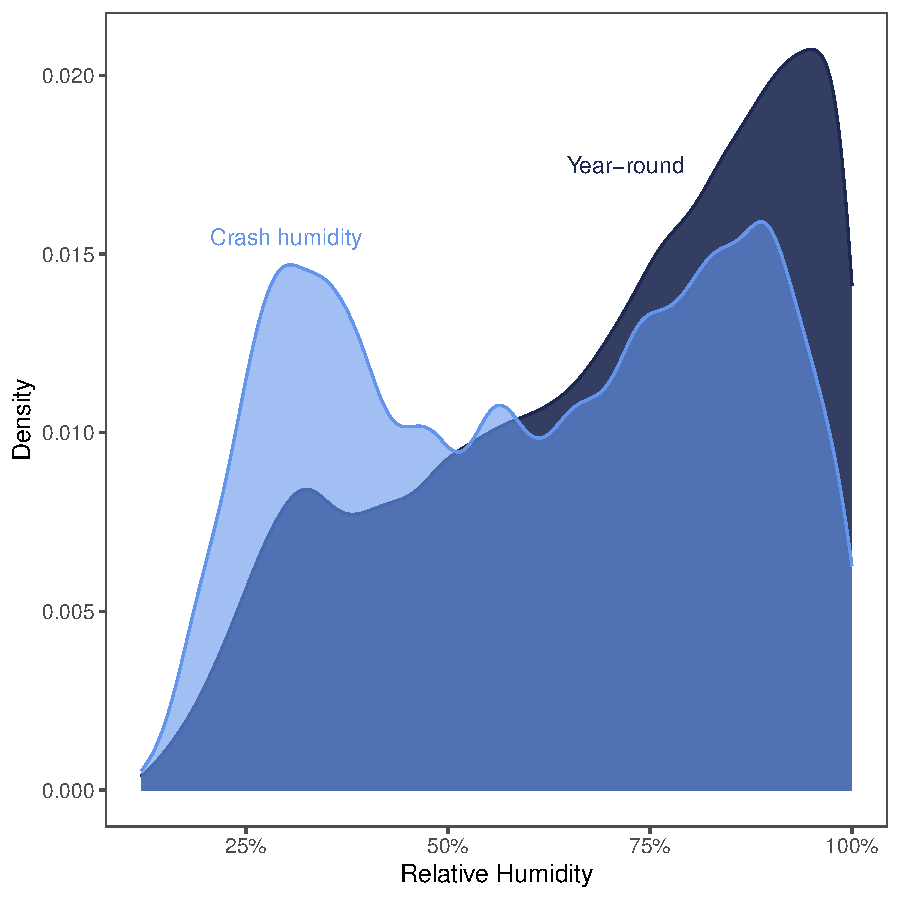
\includegraphics{variableinvestigation-010}

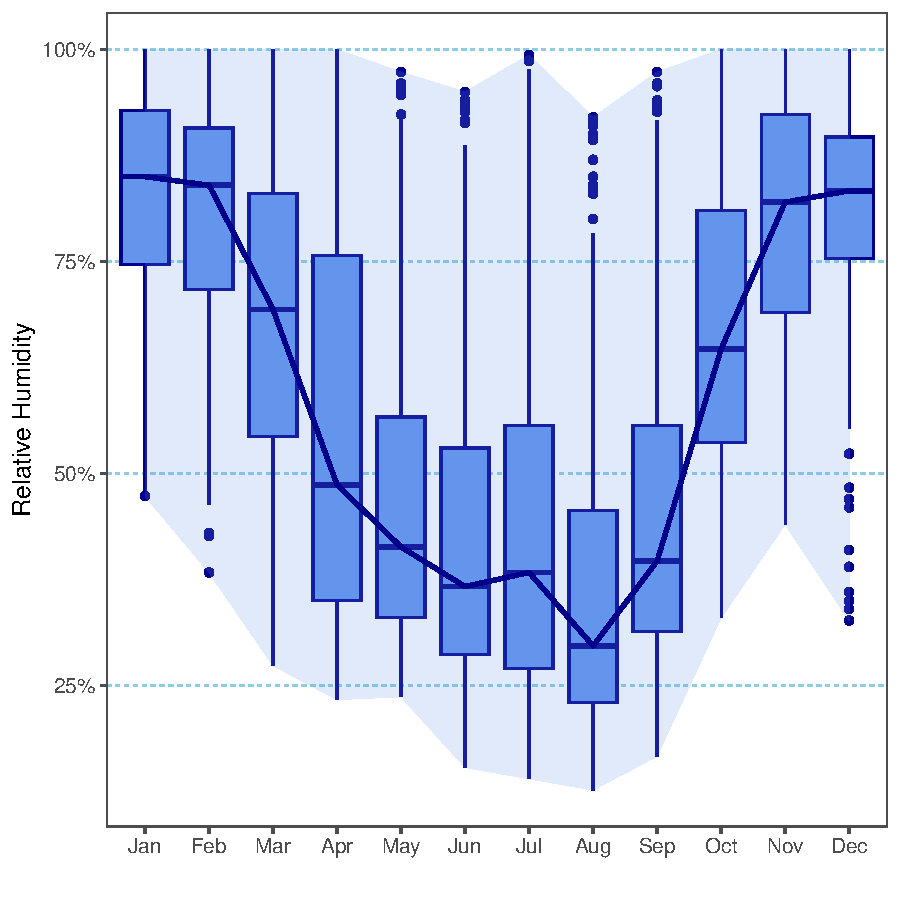
\includegraphics{variableinvestigation-011}



\pagebreak
\subsection{Precipitation}

\begin{Schunk}
\begin{Soutput}
  Avg.precipitation Avg.crash.precipitation
1        0.02998858              0.03110818
\end{Soutput}
\begin{Soutput}
Rounded table of precipitation values:
\end{Soutput}
\begin{Soutput}
    0     1     2     3     4 
54934  1105    54     1     7 
\end{Soutput}
\begin{Soutput}
Many are 0...
\end{Soutput}
\end{Schunk}
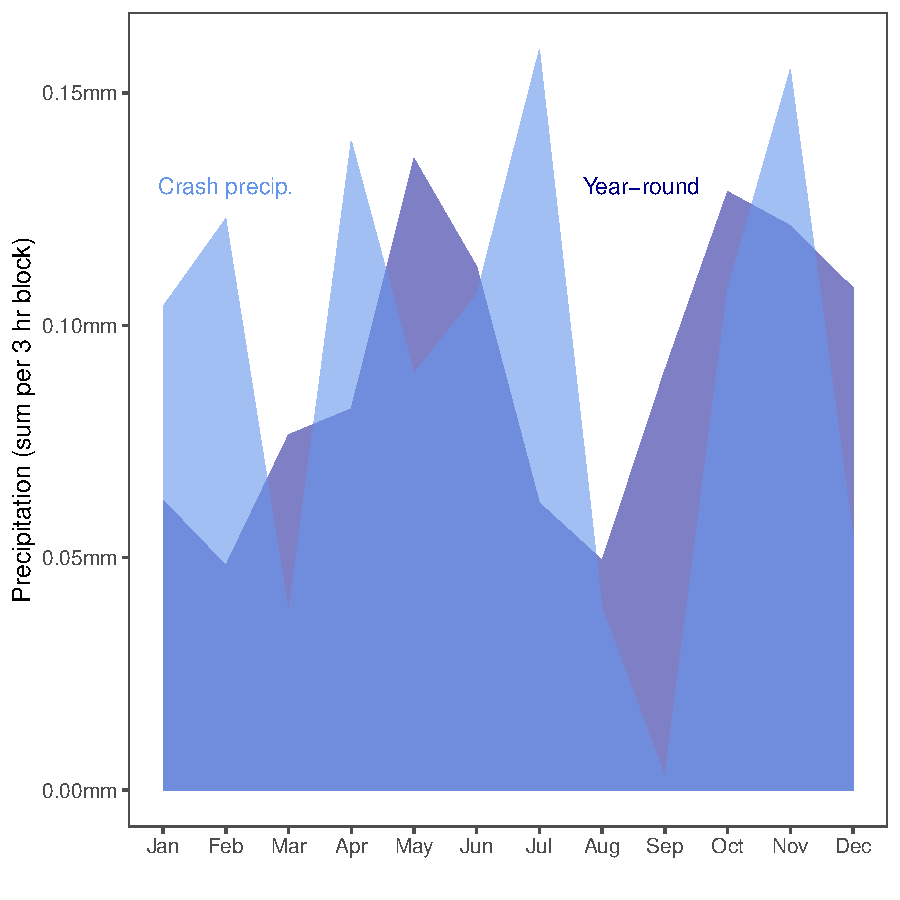
\includegraphics{variableinvestigation-012}


\pagebreak
\subsection{Wind Speed}

\begin{Schunk}
\begin{Soutput}
  Avg.wind.speed Avg.crash.wind.speed
1        8.41538             10.27689
\end{Soutput}
\end{Schunk}
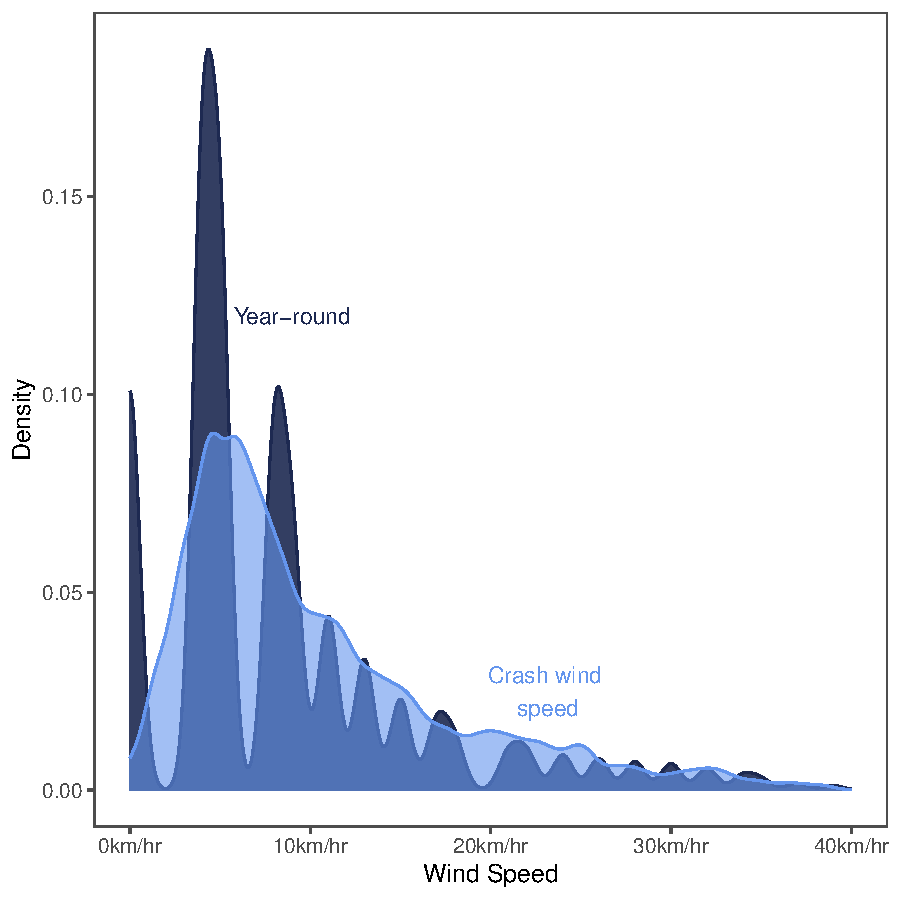
\includegraphics{variableinvestigation-013}

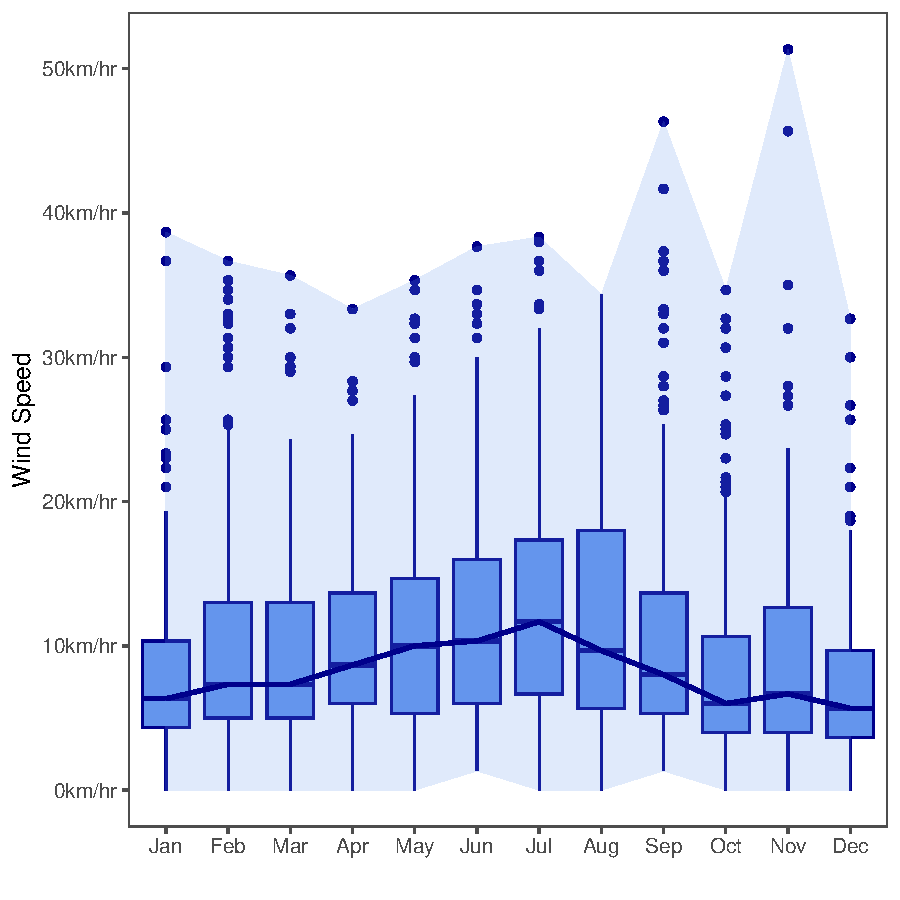
\includegraphics{variableinvestigation-014}



\pagebreak
\subsection{Wind Direction}

\begin{Schunk}
\begin{Soutput}
  Avg.wind.dir. Avg.crash.wind.dir.
1       19.1302              21.163
\end{Soutput}
\end{Schunk}
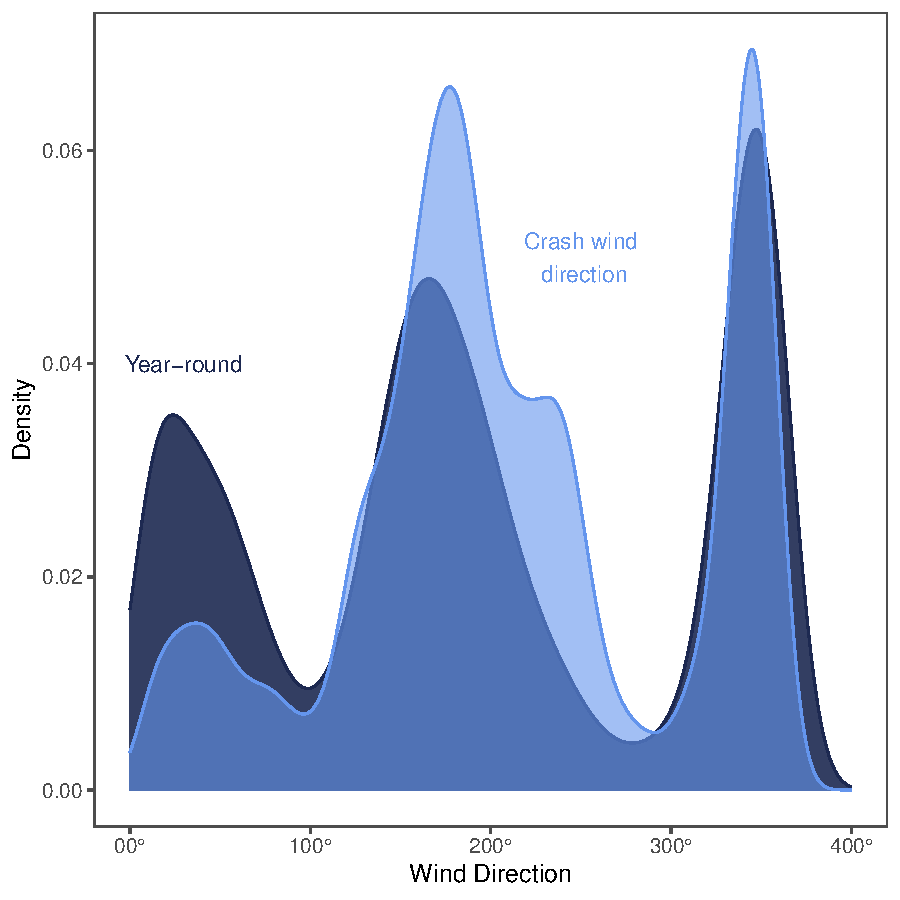
\includegraphics{variableinvestigation-015}

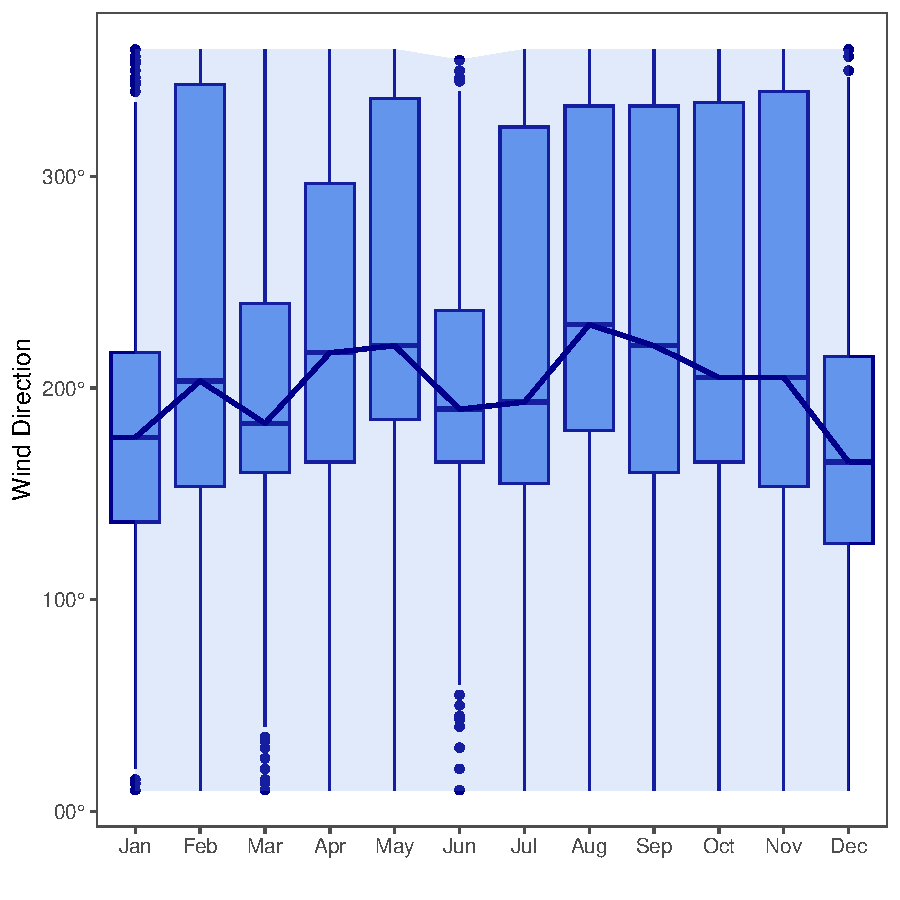
\includegraphics{variableinvestigation-016}



\pagebreak
\subsection{Visibility}

\begin{Schunk}
\begin{Soutput}
  Avg.visibility Avg.crash.visibility
1       15.10429             15.14964
\end{Soutput}
\begin{Soutput}
Very little differences in visibility...
\end{Soutput}
\begin{Soutput}
Density plot isn't helpful because cases are so spread out.
\end{Soutput}
\end{Schunk}

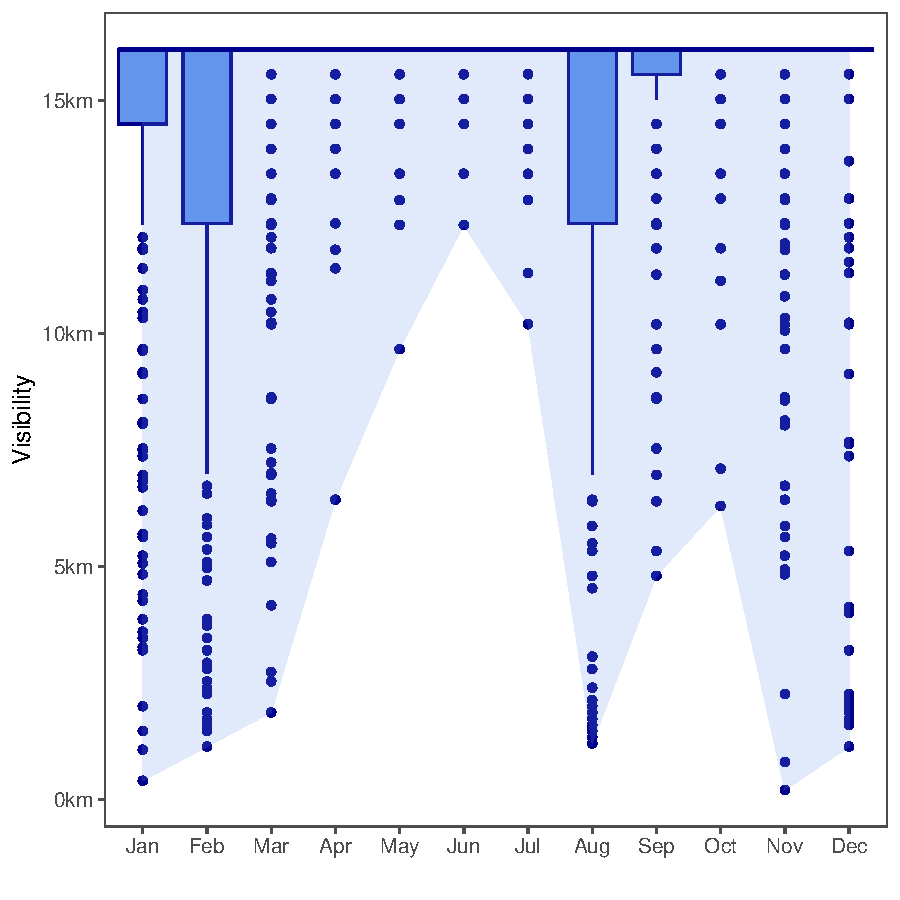
\includegraphics{variableinvestigation-018}



\pagebreak
\subsection{Air Pressure}

\begin{Schunk}
\begin{Soutput}
  Avg.air.pressure Avg.crash.air.pressure
1         96.55096               96.56156
\end{Soutput}
\end{Schunk}








\pagebreak
\section{Crash Subtypes}

\subsection{All Combined}

\begin{Schunk}
\begin{Soutput}
-----------------
Number of crashes: 56136
\end{Soutput}
\begin{Soutput}
-----------------
Number of intersection crashes: 24459 (43.6%)
\end{Soutput}
\begin{Soutput}
-----------------
Number of casualty crashes: 11473 (20.4%)
\end{Soutput}
\begin{Soutput}
-----------------
Top 5 most common streets:
\end{Soutput}
\begin{Soutput}
      HWY 97   HARVEY AVE       HWY 33    GORDON DR LAKESHORE RD 
        6019         3168         2064         1921         1372 
\end{Soutput}
\begin{Soutput}
-----------------
Avg. victims per year: 3275
\end{Soutput}
\begin{Soutput}
-----------------
Months of the year: (same as above)
\end{Soutput}
\begin{Soutput}
  JANUARY  FEBRUARY     MARCH     APRIL       MAY      JUNE      JULY    AUGUST 
     5063      4728      4120      3825      4475      4735      5152      4907 
SEPTEMBER   OCTOBER  NOVEMBER  DECEMBER 
     4632      4836      4568      5095 
\end{Soutput}
\begin{Soutput}
-----------------
Days of the week: (same as above)
\end{Soutput}
\begin{Soutput}
   SUNDAY    MONDAY   TUESDAY WEDNESDAY  THURSDAY    FRIDAY  SATURDAY 
     5464      8024      8728      8790      9061      9316      6753 
\end{Soutput}
\begin{Soutput}
-----------------
Avg. Temperature: (same as above)
\end{Soutput}
\begin{Soutput}
  Avg.temp. Avg.crash.temp.
1  8.511442        10.91872
\end{Soutput}
\begin{Soutput}
-----------------
Avg Relative Humidity: (same as above)
\end{Soutput}
\begin{Soutput}
  Avg.humidity Avg.crash.humidity
1     69.32555           60.50743
\end{Soutput}
\begin{Soutput}
-----------------
Avg. Precipitation Amount (mm): (same as above)
\end{Soutput}
\begin{Soutput}
  Avg.precipitation Avg.crash.precipitation
1        0.02998858              0.03110818
\end{Soutput}
\begin{Soutput}
-----------------
Avg. Wind Speed (km/h): (same as above)
\end{Soutput}
\begin{Soutput}
  Avg.wind.speed Avg.crash.wind.speed
1        8.41538             10.27689
\end{Soutput}
\begin{Soutput}
-----------------
Avg. Visibility (km): (same as above)
\end{Soutput}
\begin{Soutput}
  Avg.visibility Avg.crash.visibility
1       15.10429             15.14964
\end{Soutput}
\end{Schunk}




\pagebreak
\subsection{Cyclist Crashes}


\begin{Schunk}
\begin{Soutput}
-----------------
Number of crashes: 411
\end{Soutput}
\begin{Soutput}
-----------------
Number of intersection crashes: 328 (79.8%)
\end{Soutput}
\begin{Soutput}
-----------------
Number of casualty crashes: 332 (80.8%)
\end{Soutput}
\begin{Soutput}
-----------------
Top 5 most common streets:
\end{Soutput}
\begin{Soutput}
   GORDON DR LAKESHORE RD       HWY 97  BERNARD AVE       HWY 33 
          40           23           21           19           18 
\end{Soutput}
\begin{Soutput}
-----------------
Avg. victims per year: 72
\end{Soutput}
\begin{Soutput}
-----------------
Months of the year:
\end{Soutput}
\begin{Soutput}
  JANUARY  FEBRUARY     MARCH     APRIL       MAY      JUNE      JULY    AUGUST 
        2        11        18        24        45        48        53        68 
SEPTEMBER   OCTOBER  NOVEMBER  DECEMBER 
       60        36        30        16 
\end{Soutput}
\begin{Soutput}
-----------------
Days of the week:
\end{Soutput}
\begin{Soutput}
   SUNDAY    MONDAY   TUESDAY WEDNESDAY  THURSDAY    FRIDAY  SATURDAY 
       32        52        78        75        65        78        31 
\end{Soutput}
\begin{Soutput}
-----------------
Avg. Temperature:
\end{Soutput}
\begin{Soutput}
  Avg.temp. Avg.crash.temp. Avg.cyclist.crash.temp.
1  8.511442        10.91872                17.02561
\end{Soutput}
\begin{Soutput}
-----------------
Avg Relative Humidity:
\end{Soutput}
\begin{Soutput}
  Avg.humidity Avg.crash.humidity Avg.cyclist.crash.humidity
1     69.32555           60.50743                   50.07967
\end{Soutput}
\begin{Soutput}
-----------------
Avg. Precipitation Amount (mm):
\end{Soutput}
\begin{Soutput}
  Avg.precipitation Avg.crash.precipitation Avg.cyclist.crash.precipitation
1        0.02998858              0.03110818                      0.02715447
\end{Soutput}
\begin{Soutput}
-----------------
Avg. Wind Speed (km/h):
\end{Soutput}
\begin{Soutput}
  Avg.wind.speed Avg.crash.wind.speed Avg.cyclist.crash.wind.speed
1        8.41538             10.27689                     10.45772
\end{Soutput}
\begin{Soutput}
-----------------
Avg. Visibility (km):
\end{Soutput}
\begin{Soutput}
  Avg.visibility Avg.crash.visibility Avg.cyclist.crash.visibility
1       15.10429             15.14964                     15.40862
\end{Soutput}
\end{Schunk}






\pagebreak
\subsection{Animal Crashes}


\begin{Schunk}
\begin{Soutput}
-----------------
Number of crashes: 2018
\end{Soutput}
\begin{Soutput}
-----------------
Number of intersection crashes: 686 (34%)
\end{Soutput}
\begin{Soutput}
-----------------
Number of casualty crashes: 130 (6.4%)
\end{Soutput}
\begin{Soutput}
-----------------
Top 5 most common streets:
\end{Soutput}
\begin{Soutput}
      HWY 97       HWY 33  WESTSIDE RD LAKESHORE RD BOUCHERIE RD 
         366          272          194           71           52 
\end{Soutput}
\begin{Soutput}
-----------------
Avg. victims per year: 30
\end{Soutput}
\begin{Soutput}
-----------------
Months of the year:
\end{Soutput}
\begin{Soutput}
  JANUARY  FEBRUARY     MARCH     APRIL       MAY      JUNE      JULY    AUGUST 
      152       135       153       126       127       152       143       158 
SEPTEMBER   OCTOBER  NOVEMBER  DECEMBER 
      182       257       280       153 
\end{Soutput}
\begin{Soutput}
-----------------
Days of the week:
\end{Soutput}
\begin{Soutput}
   SUNDAY    MONDAY   TUESDAY WEDNESDAY  THURSDAY    FRIDAY  SATURDAY 
      244       307       284       312       303       329       239 
\end{Soutput}
\begin{Soutput}
-----------------
Avg. Temperature:
\end{Soutput}
\begin{Soutput}
  Avg.temp. Avg.crash.temp. Avg.animal.crash.temp.
1  8.511442        10.91872               8.280433
\end{Soutput}
\begin{Soutput}
-----------------
Avg Relative Humidity:
\end{Soutput}
\begin{Soutput}
  Avg.humidity Avg.crash.humidity Avg.animal.crash.humidity
1     69.32555           60.50743                  70.59081
\end{Soutput}
\begin{Soutput}
-----------------
Avg. Precipitation Amount (mm):
\end{Soutput}
\begin{Soutput}
  Avg.precipitation Avg.crash.precipitation Avg.animal.crash.precipitation
1        0.02998858              0.03110818                     0.02688812
\end{Soutput}
\begin{Soutput}
-----------------
Avg. Wind Speed (km/h):
\end{Soutput}
\begin{Soutput}
  Avg.wind.speed Avg.crash.wind.speed Avg.animal.crash.wind.speed
1        8.41538             10.27689                     8.21608
\end{Soutput}
\begin{Soutput}
-----------------
Avg. Visibility (km):
\end{Soutput}
\begin{Soutput}
  Avg.visibility Avg.crash.visibility Avg.animal.crash.visibility
1       15.10429             15.14964                    15.27789
\end{Soutput}
\end{Schunk}



\pagebreak
\subsection{Heavy Vehicle Crashes}


\begin{Schunk}
\begin{Soutput}
-----------------
Number of crashes: 2051
\end{Soutput}
\begin{Soutput}
-----------------
Number of intersection crashes: 932 (45.4%)
\end{Soutput}
\begin{Soutput}
-----------------
Number of casualty crashes: 365 (17.8%)
\end{Soutput}
\begin{Soutput}
-----------------
Top 5 most common streets:
\end{Soutput}
\begin{Soutput}
    HWY 97     HWY 33 HARVEY AVE   HWY 97 N  GORDON DR 
       310         77         73         58         47 
\end{Soutput}
\begin{Soutput}
-----------------
Avg. victims per year: 100
\end{Soutput}
\begin{Soutput}
-----------------
Months of the year:
\end{Soutput}
\begin{Soutput}
  JANUARY  FEBRUARY     MARCH     APRIL       MAY      JUNE      JULY    AUGUST 
      187       173       145       116       157       197       182       181 
SEPTEMBER   OCTOBER  NOVEMBER  DECEMBER 
      185       170       184       174 
\end{Soutput}
\begin{Soutput}
-----------------
Days of the week:
\end{Soutput}
\begin{Soutput}
   SUNDAY    MONDAY   TUESDAY WEDNESDAY  THURSDAY    FRIDAY  SATURDAY 
       56       370       378       365       380       402       100 
\end{Soutput}
\begin{Soutput}
-----------------
Avg. Temperature:
\end{Soutput}
\begin{Soutput}
  Avg.temp. Avg.crash.temp. Avg.heavy.crash.temp.
1  8.511442        10.91872              10.61056
\end{Soutput}
\begin{Soutput}
-----------------
Avg Relative Humidity:
\end{Soutput}
\begin{Soutput}
  Avg.humidity Avg.crash.humidity Avg.heavy.crash.humidity
1     69.32555           60.50743                 61.85107
\end{Soutput}
\begin{Soutput}
-----------------
Avg. Precipitation Amount (mm):
\end{Soutput}
\begin{Soutput}
  Avg.precipitation Avg.crash.precipitation Avg.heavy.crash.precipitation
1        0.02998858              0.03110818                    0.03264974
\end{Soutput}
\begin{Soutput}
-----------------
Avg. Wind Speed (km/h):
\end{Soutput}
\begin{Soutput}
  Avg.wind.speed Avg.crash.wind.speed Avg.heavy.crash.wind.speed
1        8.41538             10.27689                   9.744303
\end{Soutput}
\begin{Soutput}
-----------------
Avg. Visibility (km):
\end{Soutput}
\begin{Soutput}
  Avg.visibility Avg.crash.visibility Avg.heavy.crash.visibility
1       15.10429             15.14964                   15.04907
\end{Soutput}
\end{Schunk}



\pagebreak
\subsection{Motorcycle Crashes}


\begin{Schunk}
\begin{Soutput}
-----------------
Number of crashes: 463
\end{Soutput}
\begin{Soutput}
-----------------
Number of intersection crashes: 288 (62.2%)
\end{Soutput}
\begin{Soutput}
-----------------
Number of casualty crashes: 275 (59.4%)
\end{Soutput}
\begin{Soutput}
-----------------
Top 5 most common streets:
\end{Soutput}
\begin{Soutput}
     HWY 97  HARVEY AVE      HWY 33 WESTSIDE RD      KLO RD 
         67          22          20          13          11 
\end{Soutput}
\begin{Soutput}
-----------------
Avg. victims per year: 66
\end{Soutput}
\begin{Soutput}
-----------------
Months of the year:
\end{Soutput}
\begin{Soutput}
  JANUARY  FEBRUARY     MARCH     APRIL       MAY      JUNE      JULY    AUGUST 
        0         4        17        43        51        71        97        71 
SEPTEMBER   OCTOBER  NOVEMBER  DECEMBER 
       61        39         9         0 
\end{Soutput}
\begin{Soutput}
-----------------
Days of the week:
\end{Soutput}
\begin{Soutput}
   SUNDAY    MONDAY   TUESDAY WEDNESDAY  THURSDAY    FRIDAY  SATURDAY 
       65        49        58        57        69        90        75 
\end{Soutput}
\begin{Soutput}
-----------------
Avg. Temperature:
\end{Soutput}
\begin{Soutput}
  Avg.temp. Avg.crash.temp. Avg.motorcycle.crash.temp.
1  8.511442        10.91872                   19.28287
\end{Soutput}
\begin{Soutput}
-----------------
Avg Relative Humidity:
\end{Soutput}
\begin{Soutput}
  Avg.humidity Avg.crash.humidity Avg.motorcycle.crash.humidity
1     69.32555           60.50743                      45.53852
\end{Soutput}
\begin{Soutput}
-----------------
Avg. Precipitation Amount (mm):
\end{Soutput}
\begin{Soutput}
  Avg.precipitation Avg.crash.precipitation Avg.motorcycle.crash.precipitation
1        0.02998858              0.03110818                         0.02541397
\end{Soutput}
\begin{Soutput}
-----------------
Avg. Wind Speed (km/h):
\end{Soutput}
\begin{Soutput}
  Avg.wind.speed Avg.crash.wind.speed Avg.motorcycle.crash.wind.speed
1        8.41538             10.27689                        11.33549
\end{Soutput}
\begin{Soutput}
-----------------
Avg. Visibility (km):
\end{Soutput}
\begin{Soutput}
  Avg.visibility Avg.crash.visibility Avg.motorcycle.crash.visibility
1       15.10429             15.14964                        15.54327
\end{Soutput}
\end{Schunk}



\pagebreak
\subsection{Parked Vehicle Crashes}


\begin{Schunk}
\begin{Soutput}
-----------------
Number of crashes: 17569
\end{Soutput}
\begin{Soutput}
-----------------
Number of intersection crashes: 2790 (15.9%)
\end{Soutput}
\begin{Soutput}
-----------------
Number of casualty crashes: 353 (2%)
\end{Soutput}
\begin{Soutput}
-----------------
Top 5 most common streets:
\end{Soutput}
\begin{Soutput}
  HARVEY AVE       HWY 97 LAKESHORE RD     LOUIE DR    GORDON DR 
        1221          760          520          473          446 
\end{Soutput}
\begin{Soutput}
-----------------
Avg. victims per year: 92
\end{Soutput}
\begin{Soutput}
-----------------
Months of the year:
\end{Soutput}
\begin{Soutput}
  JANUARY  FEBRUARY     MARCH     APRIL       MAY      JUNE      JULY    AUGUST 
     1589      1415      1369      1271      1439      1566      1629      1607 
SEPTEMBER   OCTOBER  NOVEMBER  DECEMBER 
     1449      1487      1316      1432 
\end{Soutput}
\begin{Soutput}
-----------------
Days of the week:
\end{Soutput}
\begin{Soutput}
   SUNDAY    MONDAY   TUESDAY WEDNESDAY  THURSDAY    FRIDAY  SATURDAY 
     1948      2518      2615      2649      2664      2780      2395 
\end{Soutput}
\begin{Soutput}
-----------------
Avg. Temperature:
\end{Soutput}
\begin{Soutput}
  Avg.temp. Avg.crash.temp. Avg.parked.crash.temp.
1  8.511442        10.91872               11.32006
\end{Soutput}
\begin{Soutput}
-----------------
Avg Relative Humidity:
\end{Soutput}
\begin{Soutput}
  Avg.humidity Avg.crash.humidity Avg.parked.crash.humidity
1     69.32555           60.50743                  59.20128
\end{Soutput}
\begin{Soutput}
-----------------
Avg. Precipitation Amount (mm):
\end{Soutput}
\begin{Soutput}
  Avg.precipitation Avg.crash.precipitation Avg.parked.crash.precipitation
1        0.02998858              0.03110818                     0.02897205
\end{Soutput}
\begin{Soutput}
-----------------
Avg. Wind Speed (km/h):
\end{Soutput}
\begin{Soutput}
  Avg.wind.speed Avg.crash.wind.speed Avg.parked.crash.wind.speed
1        8.41538             10.27689                    10.38783
\end{Soutput}
\begin{Soutput}
-----------------
Avg. Visibility (km):
\end{Soutput}
\begin{Soutput}
  Avg.visibility Avg.crash.visibility Avg.parked.crash.visibility
1       15.10429             15.14964                     15.1956
\end{Soutput}
\end{Schunk}



\pagebreak
\subsection{Pedestrian Crashes}


\begin{Schunk}
\begin{Soutput}
-----------------
Number of crashes: 346
\end{Soutput}
\begin{Soutput}
-----------------
Number of intersection crashes: 220 (63.6%)
\end{Soutput}
\begin{Soutput}
-----------------
Number of casualty crashes: 289 (83.5%)
\end{Soutput}
\begin{Soutput}
-----------------
Top 5 most common streets:
\end{Soutput}
\begin{Soutput}
HARVEY AVE  GORDON DR     HWY 97     HWY 33   BANKS RD 
        26         22         22         12         11 
\end{Soutput}
\begin{Soutput}
-----------------
Avg. victims per year: 69
\end{Soutput}
\begin{Soutput}
-----------------
Months of the year:
\end{Soutput}
\begin{Soutput}
  JANUARY  FEBRUARY     MARCH     APRIL       MAY      JUNE      JULY    AUGUST 
       35        13        21        19        27        28        28        32 
SEPTEMBER   OCTOBER  NOVEMBER  DECEMBER 
       34        40        33        36 
\end{Soutput}
\begin{Soutput}
-----------------
Days of the week:
\end{Soutput}
\begin{Soutput}
   SUNDAY    MONDAY   TUESDAY WEDNESDAY  THURSDAY    FRIDAY  SATURDAY 
       33        44        39        66        57        65        42 
\end{Soutput}
\begin{Soutput}
-----------------
Avg. Temperature:
\end{Soutput}
\begin{Soutput}
  Avg.temp. Avg.crash.temp. Avg.pedestrian.crash.temp.
1  8.511442        10.91872                   10.77013
\end{Soutput}
\begin{Soutput}
-----------------
Avg Relative Humidity:
\end{Soutput}
\begin{Soutput}
  Avg.humidity Avg.crash.humidity Avg.pedestrian.crash.humidity
1     69.32555           60.50743                      63.38247
\end{Soutput}
\begin{Soutput}
-----------------
Avg. Precipitation Amount (mm):
\end{Soutput}
\begin{Soutput}
  Avg.precipitation Avg.crash.precipitation Avg.pedestrian.crash.precipitation
1        0.02998858              0.03110818                         0.03121387
\end{Soutput}
\begin{Soutput}
-----------------
Avg. Wind Speed (km/h):
\end{Soutput}
\begin{Soutput}
  Avg.wind.speed Avg.crash.wind.speed Avg.pedestrian.crash.wind.speed
1        8.41538             10.27689                        9.628131
\end{Soutput}
\begin{Soutput}
-----------------
Avg. Visibility (km):
\end{Soutput}
\begin{Soutput}
  Avg.visibility Avg.crash.visibility Avg.pedestrian.crash.visibility
1       15.10429             15.14964                        15.20434
\end{Soutput}
\end{Schunk}









\pagebreak
\section{}






\end{document}
